%%%%%%%%%%%%%%%%%%%%%%%%%%%%%%%%%%%%%%%%%
% Journal Article
% LaTeX Template
% Version 1.3 (9/9/13)
%
% This template has been downloaded from:
% http://www.LaTeXTemplates.com
%
% Original author:
% Frits Wenneker (http://www.howtotex.com)
%
% License:
% CC BY-NC-SA 3.0 (http://creativecommons.org/licenses/by-nc-sa/3.0/)
%
%%%%%%%%%%%%%%%%%%%%%%%%%%%%%%%%%%%%%%%%%

%----------------------------------------------------------------------------------------
%	PACKAGES AND OTHER DOCUMENT CONFIGURATIONS
%----------------------------------------------------------------------------------------

\documentclass[twoside]{article}

\usepackage[pdftex]{graphicx}
\usepackage{amsmath}
\usepackage{amssymb}

\usepackage{lipsum} % Package to generate dummy text throughout this template

\usepackage[sc]{mathpazo} % Use the Palatino font
\usepackage[T1]{fontenc} % Use 8-bit encoding that has 256 glyphs
\linespread{1.05} % Line spacing - Palatino needs more space between lines
\usepackage{microtype} % Slightly tweak font spacing for aesthetics

\usepackage[hmarginratio=1:1,top=32mm,columnsep=20pt]{geometry} % Document margins
\usepackage{multicol} % Used for the two-column layout of the document
\usepackage[hang, small,labelfont=bf,up,textfont=it,up]{caption} % Custom captions under/above floats in tables or figures
\usepackage{booktabs} % Horizontal rules in tables
\usepackage{float} % Required for tables and figures in the multi-column environment - they need to be placed in specific locations with the [H] (e.g. \begin{table}[H])
\usepackage{hyperref} % For hyperlinks in the PDF

\usepackage{lettrine} % The lettrine is the first enlarged letter at the beginning of the text
\usepackage{paralist} % Used for the compactitem environment which makes bullet points with less space between them

\usepackage{abstract} % Allows abstract customization
\renewcommand{\abstractnamefont}{\normalfont\bfseries} % Set the "Abstract" text to bold
\renewcommand{\abstracttextfont}{\normalfont\small\itshape} % Set the abstract itself to small italic text

\usepackage{titlesec} % Allows customization of titles
\renewcommand\thesection{\Roman{section}} % Roman numerals for the sections
\renewcommand\thesubsection{\Roman{subsection}} % Roman numerals for subsections
\titleformat{\section}[block]{\large\scshape\centering}{\thesection.}{1em}{} % Change the look of the section titles
\titleformat{\subsection}[block]{\large}{\thesubsection.}{1em}{} % Change the look of the section titles

\usepackage{fancyhdr} % Headers and footers
\pagestyle{fancy} % All pages have headers and footers
\fancyhead{} % Blank out the default header
\fancyfoot{} % Blank out the default footer
\fancyhead[C]{} % Custom header text
\fancyfoot[RO,LE]{\thepage} % Custom footer text

%----------------------------------------------------------------------------------------
%	TITLE SECTION
%----------------------------------------------------------------------------------------

\title{\vspace{-15mm}\fontsize{24pt}{10pt}\selectfont\textbf{Deriving a white-box model of the drive of a RC-Car using Prediction-Error-Method}} % Article title

\author{
\large
\textsc{Johannes Scherle}\thanks{A thank you or further information}\\[2mm] % Your name
\normalsize University of Freiburg \\ % Your institution
\normalsize \href{mailto:johannes.scherle@gmail.com}{johannes.scherle@gmail.com} % Your email address
\vspace{-5mm}
}
\date{}

%----------------------------------------------------------------------------------------

\begin{document}

\maketitle 

\thispagestyle{fancy} % All pages have headers and footers

%----------------------------------------------------------------------------------------
%	ABSTRACT
%----------------------------------------------------------------------------------------

%\begin{abstract}
%
%\noindent 
%
%In this project a model for the drive of a RC-Car has been derived. The aim was to model the speed of the rear wheels in dependency of an input PWM-Signal into a brushless motor. Step responses for different input signals were measured. Based on these measurements an ARX-Model was derived using the Prediction-Error-Method. It has showed, that this linear model was not suitable for describing the nonlinear behavior of the drive. Therefore the linear model was modified by mapping the input PWM-Signals with a nonlinear function. Thus, a signficantly better match of the model to the measured data could be achieved.
%
%\end{abstract}

%----------------------------------------------------------------------------------------
%	ARTICLE CONTENTS
%----------------------------------------------------------------------------------------

%\begin{multicols}{2} % Two-column layout throughout the main article text

\section{Introduction}

\lettrine[nindent=0em,lines=3]{M} odel-Driven-Development is a method, often used in the development of embedded systems in which a system, that is supposed to interact with a physical enviroment is simulated with a PC before it is finally tested in real life. For this technique it is of course necessary to have a model of the physical enviroment. In this project the drive of an RC-Car which is used for students projects such as developing driver-assistance systems is modelled. The aim was to derive a model-equation, that describes the speed of the rear wheels which are driven by brushless motor in dependence of different input signals to the brushless motor.

%------------------------------------------------

\section{Experimental-setup}
The input signal was created by a remote control that sends information of the users throttle input to a reciever on the car, which modulates this information into a corresponding PWM-Signal. The PWM-Signals for different throttle positions were determined by measuring the pulse-width with an osciloscope. The signal width in the neutral position was 1,5 ms. In the following with PWM-Signal, the difference to that neutral signal is meant. The PWM-Signal is fed into the controller of a brushless motor, which then drives the wheels. The RC-Car is equipped with magnetic speed sensors on all four wheels. Using an Arduino Microcontroller step responses to different input-PWM-Signals were measured. During the experiment the car was lifted, so that the wheels were rotating freely in the air. The sample rate was 8.5 ms.


%------------------------------------------------

\section{Results and modelling}
The results of the measured step responses for different input-signals where used as input and output data. To model the system an ARX-Model of order 2, whicht is described in formula 1, was used in the first iteration. The aim was to estimate the coefficents a and b. For this purpose the matlab function arx\_pem, which was provided in the modelling and system identification lecture was used with the input data of the step response of the PWM-Signal with 120 $\mu s$. After the parameters were estimated a continuous-time transfer function was used to simulate the system. The results of the simulation, compared to the measured data can be seen in figure 2.

\begin{align}
y(k) + \sum_{i=1}^n a_i y(k - i) = \sum_{i=1}^n b_i u(k - i)
\end{align}

\begin{figure}[h!]
\begin{minipage}{0.5\textwidth}
\centering
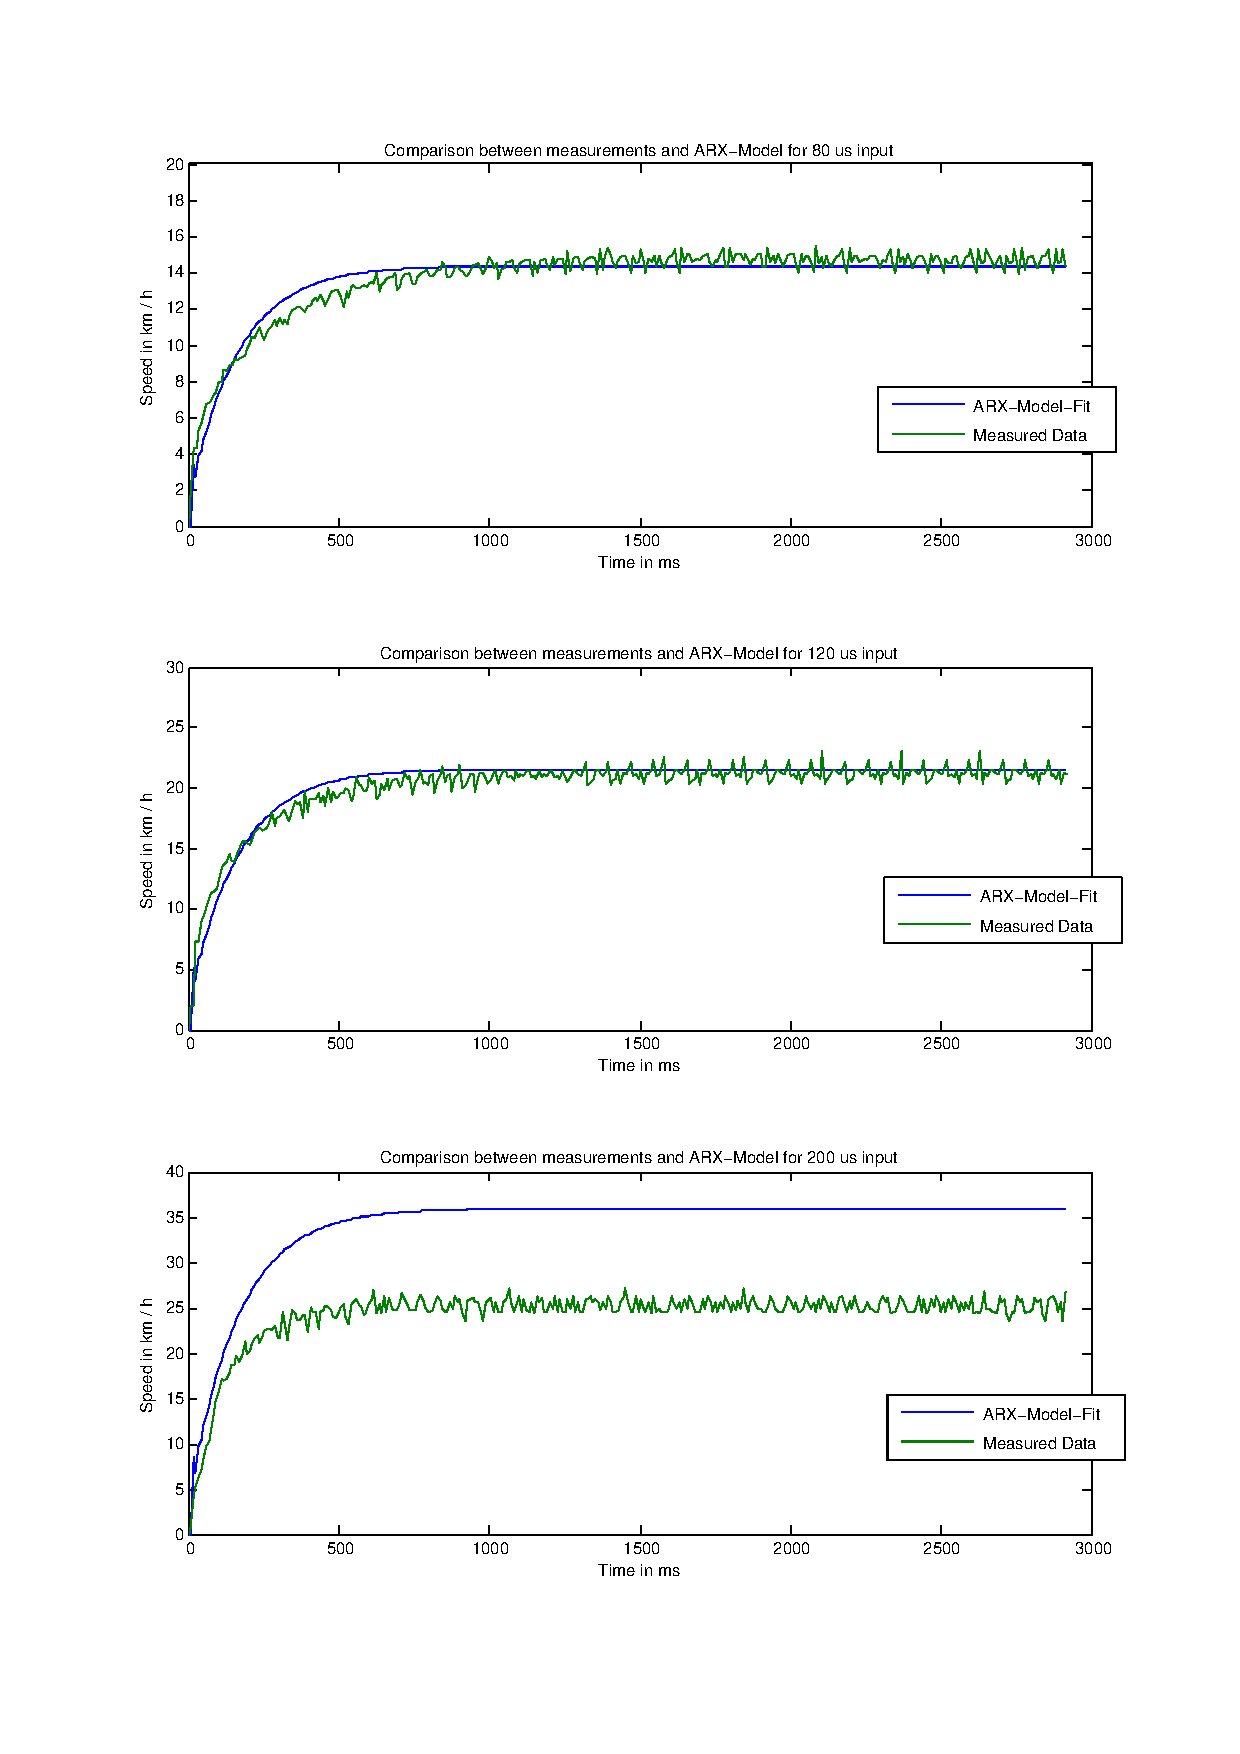
\includegraphics[scale=0.4]{comparison1.pdf}
\caption{Comparison of the measured data with the ARX-Model-Fit}
\end{minipage}
\begin{minipage}{0.5\textwidth}
\centering
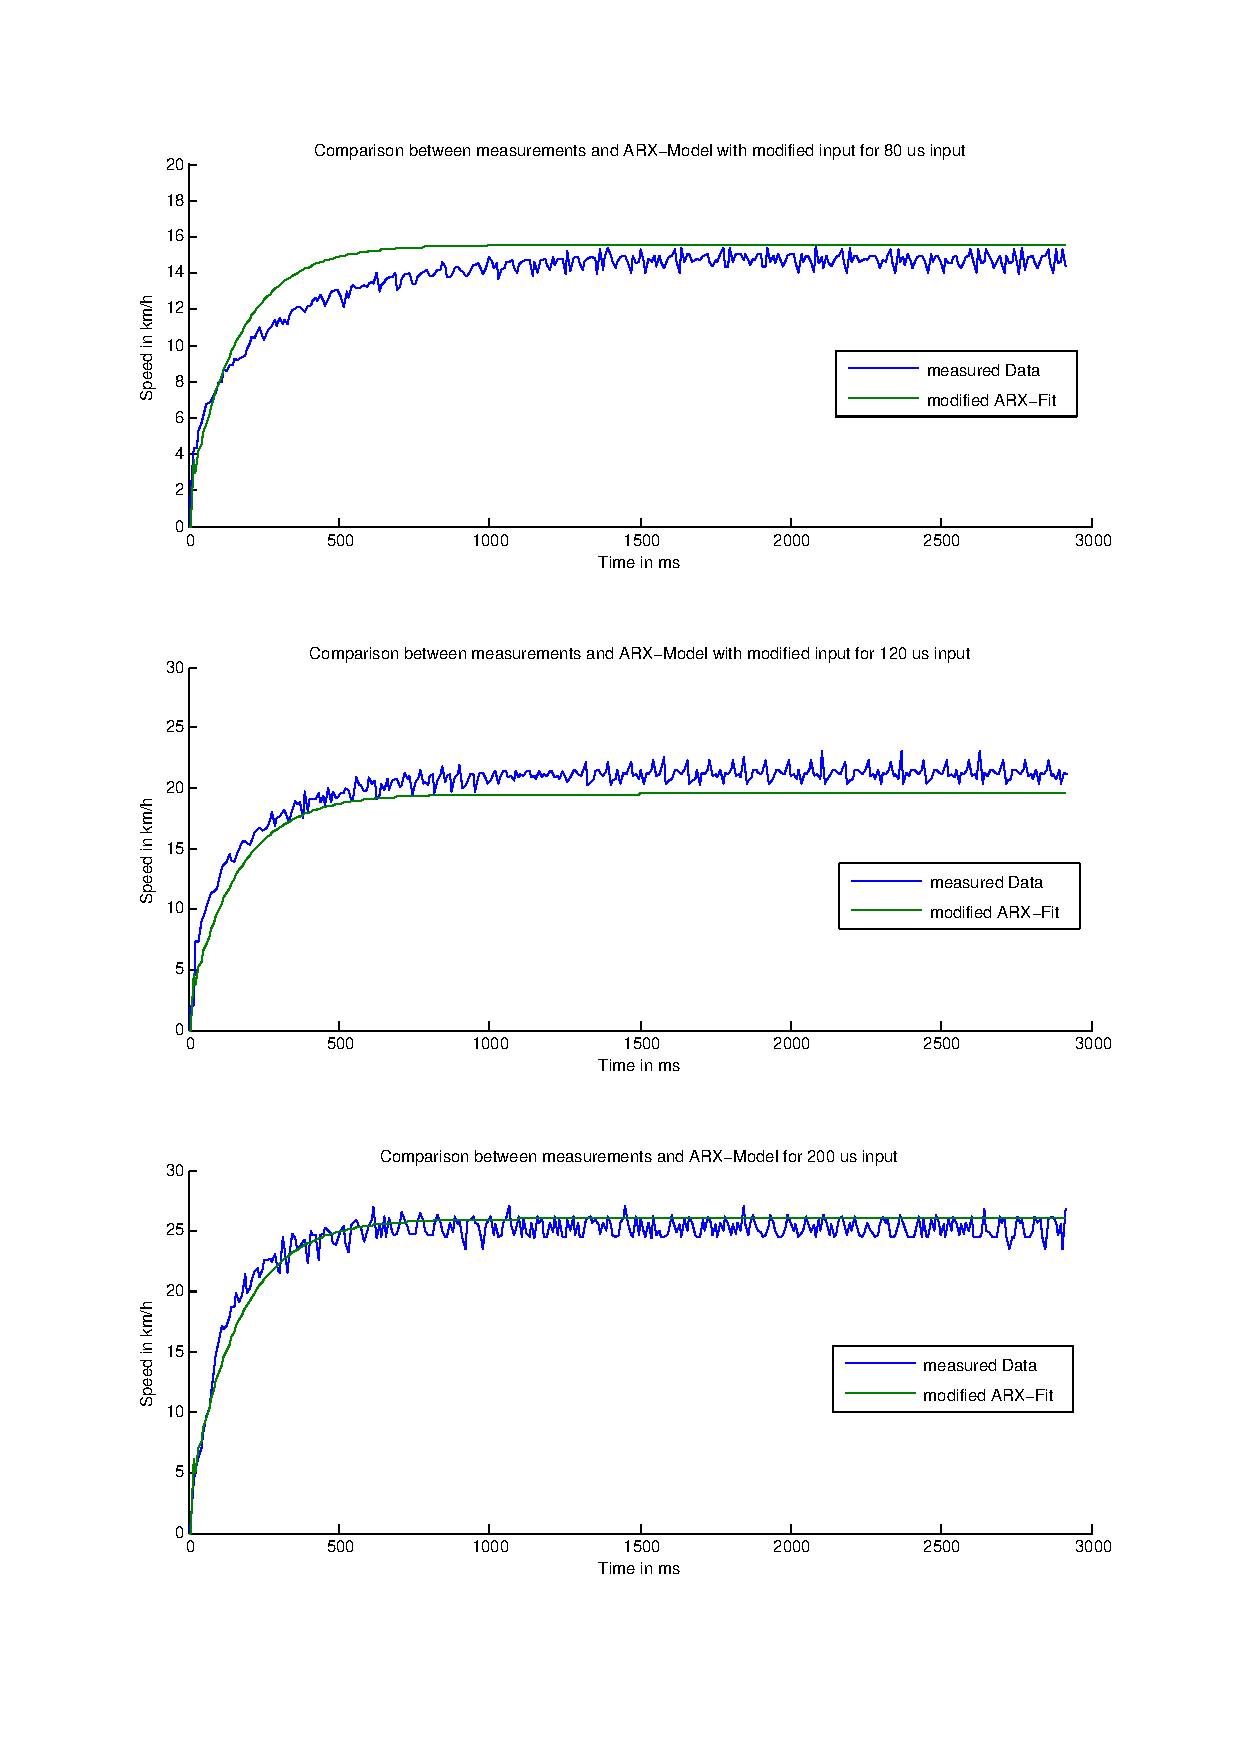
\includegraphics[scale=0.4]{comparison2.pdf}
\caption{Comparison of the measured data with the modified ARX-Model-Fit}
\end{minipage}
\end{figure}
As one can see, the simulation using an ARX-Model fits nicely for the 80 and 120 $\mu s$ PWM-Signal. However, the fit holds hardly for the 200 $\mu s$ input. This is due to the nonlinearity of the output-signal to the input signal. After the steady state was analyzed for different it showed, that the relation showed a curve which had the form of a logarithmic- or root-function. The idea then was to modify the input signals in a way that the input signal was "flattened out" for higher inputs. This was done using a root function like described in formula 2. In this function the parameter $\alpha$ and $\beta$ had to be found. A function was set up, to calculate the residual between the a simulation using a modified input signal with a given system. This function was then minimized with the lsqnonlin-function. In figure 2 again the simulation with the modified PWM-Signal is shown. It shows that using the modification of the input-signal yields a much better matching of the simulation to the measured data.
\begin{align}
modifiedPWM = \alpha \sqrt[\beta]{inputPWM}
\end{align}


%----------------------------------------------------------------------------------------
%	REFERENCE LIST
%----------------------------------------------------------------------------------------

%\begin{thebibliography}{99} % Bibliography - this is intentionally simple in this template
%
%\bibitem[Figueredo and Wolf, 2009]{Figueredo:2009dg}
%Figueredo, A.~J. and Wolf, P. S.~A. (2009).
%\newblock Assortative pairing and life history strategy - a cross-cultural
%  study.
%\newblock {\em Human Nature}, 20:317--330.
% 
%\end{thebibliography}

%----------------------------------------------------------------------------------------

%\end{multicols}

\end{document}
